

\begin{figure}[t!]
\centering
\begin{tabular}{c|c|c|}
 \multicolumn{1}{c}{~} & \multicolumn{1}{c}{H}  &  \multicolumn{1}{c}{T}\\\cline{2-3}
H &  1  &  0\\\cline{2-3}
T  & 0  &  1\\\cline{2-3}
\end{tabular}
~~~~~~~~~
\begin{tabular}{c|c|c|}
 \multicolumn{1}{c}{~} & \multicolumn{1}{c}{A}  &  \multicolumn{1}{c}{B}\\\cline{2-3}
a &  0  &  1\\\cline{2-3}
b & -1  &  0\\\cline{2-3}
\end{tabular}
\caption{Matrix games of Matching Pennies (left), and one with a pure Nash equilibrium (right).
Payoffs to the row player are shown. \label{fig:egMatrixGames}}
\end{figure}

A finite game with simultaneous moves (also called Markov games) and chance events can be described
by a tuple $(\cN, \cS = \cD\cup\cC\cup\cZ, \cA, \cT, \Delta_\star, u_i, s_0)$.
The player set $\cN = \{ 1, 2, \star \}$ contains player labels, where
$\star$ denotes the chance player, and by convention a player is denoted $i \in \cN$.
$\cS$ is a set of states, with $\cZ$ denoting the terminal states, $\cD$ the states where players make decisions,
and $\cC$ the possibly empty set of states where chance events occur. $\cA = \cA_1 \times \cA_2$ is the set of
joint actions of individual players. We denote $\cA_i(s)$ the actions available to player $i$ in state $s \in \cS$ \reviewchange{and denote the number of actions $|\cA_i(s)|$ as the \emph{branching factor for player $i$}. When player is not specified, we are talking about branching factor of all players and number of joint actions $|\cA|$.}
The transition function $\cT : \cS \times \cA_1 \times \cA_2 \mapsto \cS$ defines the successor state given a current
state and actions for both players. $\Delta_\star:\cC \mapsto \Delta(\cS)$ describes a probability distribution over
possible successor states of the chance event.
\reviewchange{Induced by $\Delta_\star$, we also define
$\cP_\star(s, r, c, s')$ as the probability of transitioning to $s'$ after choosing joint action $(r,c)$ from $s$, or
simply $1$ when $\cT(s, r, c) \not\in \cC$.}
The utility functions $u_i : \cZ \mapsto [v_{\min}, v_{\max}] \subseteq \mathbb{R}$ gives the utility of player $i$, with
$v_{min}$ and $v_{\max}$ denoting the minimum and maximum possible utility respectively. We assume constant-sum
games: $\forall z \in \cZ, u_1(z) = k - u_2(z)$.
The game begins in an initial state $s_0$.
An example of such game is depicted in Figure~\ref{fig:example} (more examples can be found in \cite[Chapter 5]{Saffidine2013thesis}).

\begin{figure}[t!]
\centering
\begin{subfigure}{12cm}
\centering
\includegraphics[width=8.0cm]{figures/tree}\\
%\includegraphics[width=10.0cm]{figures/goof3}\\
\end{subfigure}%\\
\caption{An example of a two-player simultaneous game without chance nodes which has Matching Pennies as a subgame. %, and a portion of 3-card Goofspiel including chance nodes (bottom).
The dark squares are terminal states. The values shown are optimal values that could be obtained by backward induction.\\
%bbosansky: if that's ok, I have removed the goofspiel figure since I do not think it is specifically referenced anywhere and we do not need to figures. Plus, since we do not specifically experiment with games with chance nodes, it is better not to include the figure :)
\label{fig:example}}
\end{figure}
In two-player constant sum games a (subgame perfect) Nash equilibrium strategy is often considered to be optimal. It guarantees an expected payoff of at least $V$ against any opponent. Any non-equilibrium strategy has its nemesis, which makes it win less
than $V$ in expectation. Moreover, subgame perfect Nash equilibrium strategy can earn more than $V$ against weak opponents. After the
opponent makes a sub-optimal move, the strategy will never allow it to gain the loss back.
The value $V$ is known as the minimax-optimal value of the game
and is the same for every equilibrium profile by von Neumann's minimax theorem.


A {\it matrix game} is a single step simultaneous move game with action sets $\cA_1$ and $\cA_2$.
Each entry in the matrix $A_{rc}$ where $(r,c) \in \cA_1 \times \cA_2$ corresponds to a payoff (to player 1) if row $r$ is
chosen by player 1 and column $c$ by player 2.
For example, in Matching Pennies in the left side of Figure~\ref{fig:egMatrixGames}, each player has two actions (heads or tails).
The row player receives a payoff of 1
if both players choose the same action and 0 if they do not match.
Two-player simultaneous move games are sometimes called {\it stacked matrix games} because at every state
$s$ there is a joint action set $\cA_1(s) \times \cA_2(s)$ that either leads to a terminal state or (possibly after a
chance transition) to a subgame which is itself another stacked matrix game.
In the matrix game on the right of Figure~\ref{fig:egMatrixGames}, $b$ and $B$ are strictly dominated, leaving $(a,A)$ as a
pure and only Nash equilibrium (NE) strategy.

A {\it behavioral strategy} for player $i$ is a mapping from states $s \in \cS$
to a probability distribution over the actions $\cA_i(s)$, denoted $\sigma_i(s)$.
\reviewchange{We denote $\sigma_i(s,a)$ as the probability that strategy $\sigma$ assigns to $a$ in $s$.
These strategies are often called {\it randomized}, or {\it mixed} because they represent a mixture over {\it pure} strategies, each of
which is a point in the Cartesian product space $\times_{s \in \cS} \cA_i(s)$.\footnote{\reviewchange{Notice that a pure strategy is also a mixed strategy that assigns probability 1 to a single pure strategy and probability 0 to every other pure strategy. However, as is common in the literature, we sometimes refer to a mixed strategy
to specifically mean not a pure strategy. This is mostly clear from the context, but we will clarify where necessary.}}}
\reviewchange{Let $\cH$ be a global set of histories (sequences of actions from the start of the game).}
Given a profile $\sigma = (\sigma_1, \sigma_2)$, define the probability of reaching a history $h$ under $\sigma$ as
$\pi^\sigma(h) = \pi^\sigma_1(h) \pi^\sigma_2(h) \pi^\sigma_\star(h)$, where each $\pi^\sigma_i(h)$ is a product of probabilities of the actions taken
by player $i$ along the path to $h$ ($\pi_\star$ being chance's probabilities).
Finally, define $\Sigma_i$ to be the set of behavioral strategies for player $i$.

\reviewchange{For the remainder of the article, we adopt a standard convention that the index $-i$ refers to all players except $i$.
In a game with chance events, then the $-i$ also includes the chance player, so \eg if $i = 1$ then $\pi^\sigma_{-i}(h) = \pi^\sigma_2(h) \pi^\sigma_\star(h)$.
Whereas, in the case of a matrix game, $\cA_{-i} = \cA_{3-i}$.\bbosansky{@Marc -- in exact algorithms, $-i$ is used to denote the opponent excluding the chance (chance is handled separately). How is it in sampling algorithms? I think, that it is the same there as well, no?}

There are three important concepts used in the paper that deserve explicit definition. These concepts are used to define
optimal behavior for this class of games, metrics for evaluation, and within the algorithms as well.

\begin{definition}[Dominated Action]
In a matrix game, an action $a_i \in \cA_i$ is dominated if $\forall a_{-i} \in \cA_{-i}, \forall a_i' \in \Sigma_i \setminus \{ a_i \}: u(a_i, a_{-i}) < u(a_i', a_{-i})$.
\end{definition}

No rational player would want to play a dominated action, because there is always a better one to play instead, for any action used by the opponent. The concept also
extends natrually to behavioral strategies.

\begin{definition}[Best Response]
Suppose $\sigma_{-i} \in \Sigma_{-i}$ is a fixed oppenent strategy. Define the set of best response strategies
$BR_i(\sigma_{-i}) = \{ \sigma_i~|~u(\sigma_i, \sigma_{-i}) = \max_{\sigma_i' \in \Sigma_i} u(\sigma_i', \sigma_{-i})) \}$.
A single strategy in this set, \eg $\sigma_i \in BR_i(\sigma_{-i})$, is called a best response strategy to $\sigma_{-i}$.
\end{definition}

Note that a best response can be a mixed strategy, but a pure best response always exists and is often easier to compute.

\begin{definition}[Nash Equilibrium]
A strategy profile $(\sigma_i, \sigma_{-i})$ is a Nash equilibrium profile if and only if $\sigma_i \in BR_i(\sigma_{-i})$
and $\sigma_{-i} \in BR_{-i}(\sigma_i)$.
\end{definition}

In other words, in a Nash equilibrium profile each strategy is a best response to the opponents' strategies. In two-player, zero-sum
games the set of Nash equilibria corresponds to the set of minimax-optimal strategies. That is,} a Nash equilibrium profile is
also pair of behavioral strategies optimizing
\begin{equation}\label{eq:ne}
V = \max_{\sigma_1 \in \Sigma_1} \min_{\sigma_2 \in \Sigma_2} \bE_{z \sim \sigma}[u_1(z)]
  = \max_{\sigma_1 \in \Sigma_1} \min_{\sigma_2 \in \Sigma_2} \sum_{z \in \cZ} \pi^\sigma(z) u_1(z).
\end{equation}
None of the players can improve their utility by deviating unilaterally.
For example, the Matching Pennies matrix game has a single state and the only equilibrium strategy is to mix equally between
both actions, \ie both players play with a mixed strategy $\sigma_i = \sigma_{-i} = (0.5, 0.5)$ giving an expected payoff of
$V = 0.5$.
Note that using a mixed strategy is necessary in this game to achieve a guaranteed payoff of $V$.
Any pure strategy of one player can be exploited by the opponent; \reviewchange{so while a pure best response to a fixed strategy always
exists, it is not always possible to find a Nash equilibrium for which both strategies are pure.}
For the same reason, randomized strategies are often necessary also in the multi-stage simultaneous move games.
If the strategies also optimize Equation \ref{eq:ne} in each subgame starting in an arbitrary state, the equilibrium strategy
is termed {\it subgame perfect.}

A two-player simultaneous move game is a specific type of two-player imperfect information extensive-form game.
In imperfect information
%\footnote{In this paper, we use the term {\it imperfect information} to refer to games that have situations
%where one player knows something that some of the other players do not know. However, every player knows which game they are playing,
%the distribution of chance event outcomes, and every player's utility function. This is in contrast to
%{\it imcomplete information} games in which players may also not know (or be fully certain of) the utility functions of their opponents
%or precisely how nature affects the game.}
games, states are grouped into {\it information sets}: two states $s, s' \in I$ if the player
to act at $I$ cannot distinguish which of these states the game is currently in. Any simultaneous move game can be modeled
using information sets to represent a half-completed transition, \ie $\cT(s, a_1, ?)$ or $\cT(s, ?, a_2)$.
For example, the matrix game of Rock, Paper, Scissors can be thought of as a two-step process where the first player commits
to a choice, writing it on a face-down piece of paper, and then second player responds. Figure~\ref{fig:rps-equiv} shows this
transformation, which can generally be applied to every state in a simultaneous move game by placing the root of subgame following
both players' decisions, or a successor chance node outcome.
Therefore, algorithms intended for two-player zero-sum imperfect information games may also be applied to the
simultaneous move game's equivalent extensive form.

\begin{figure}
\begin{center}
\begin{tabular}{ccc}
\includegraphics[scale=1.3]{figures/rps-nfg} & ~~~~~ & 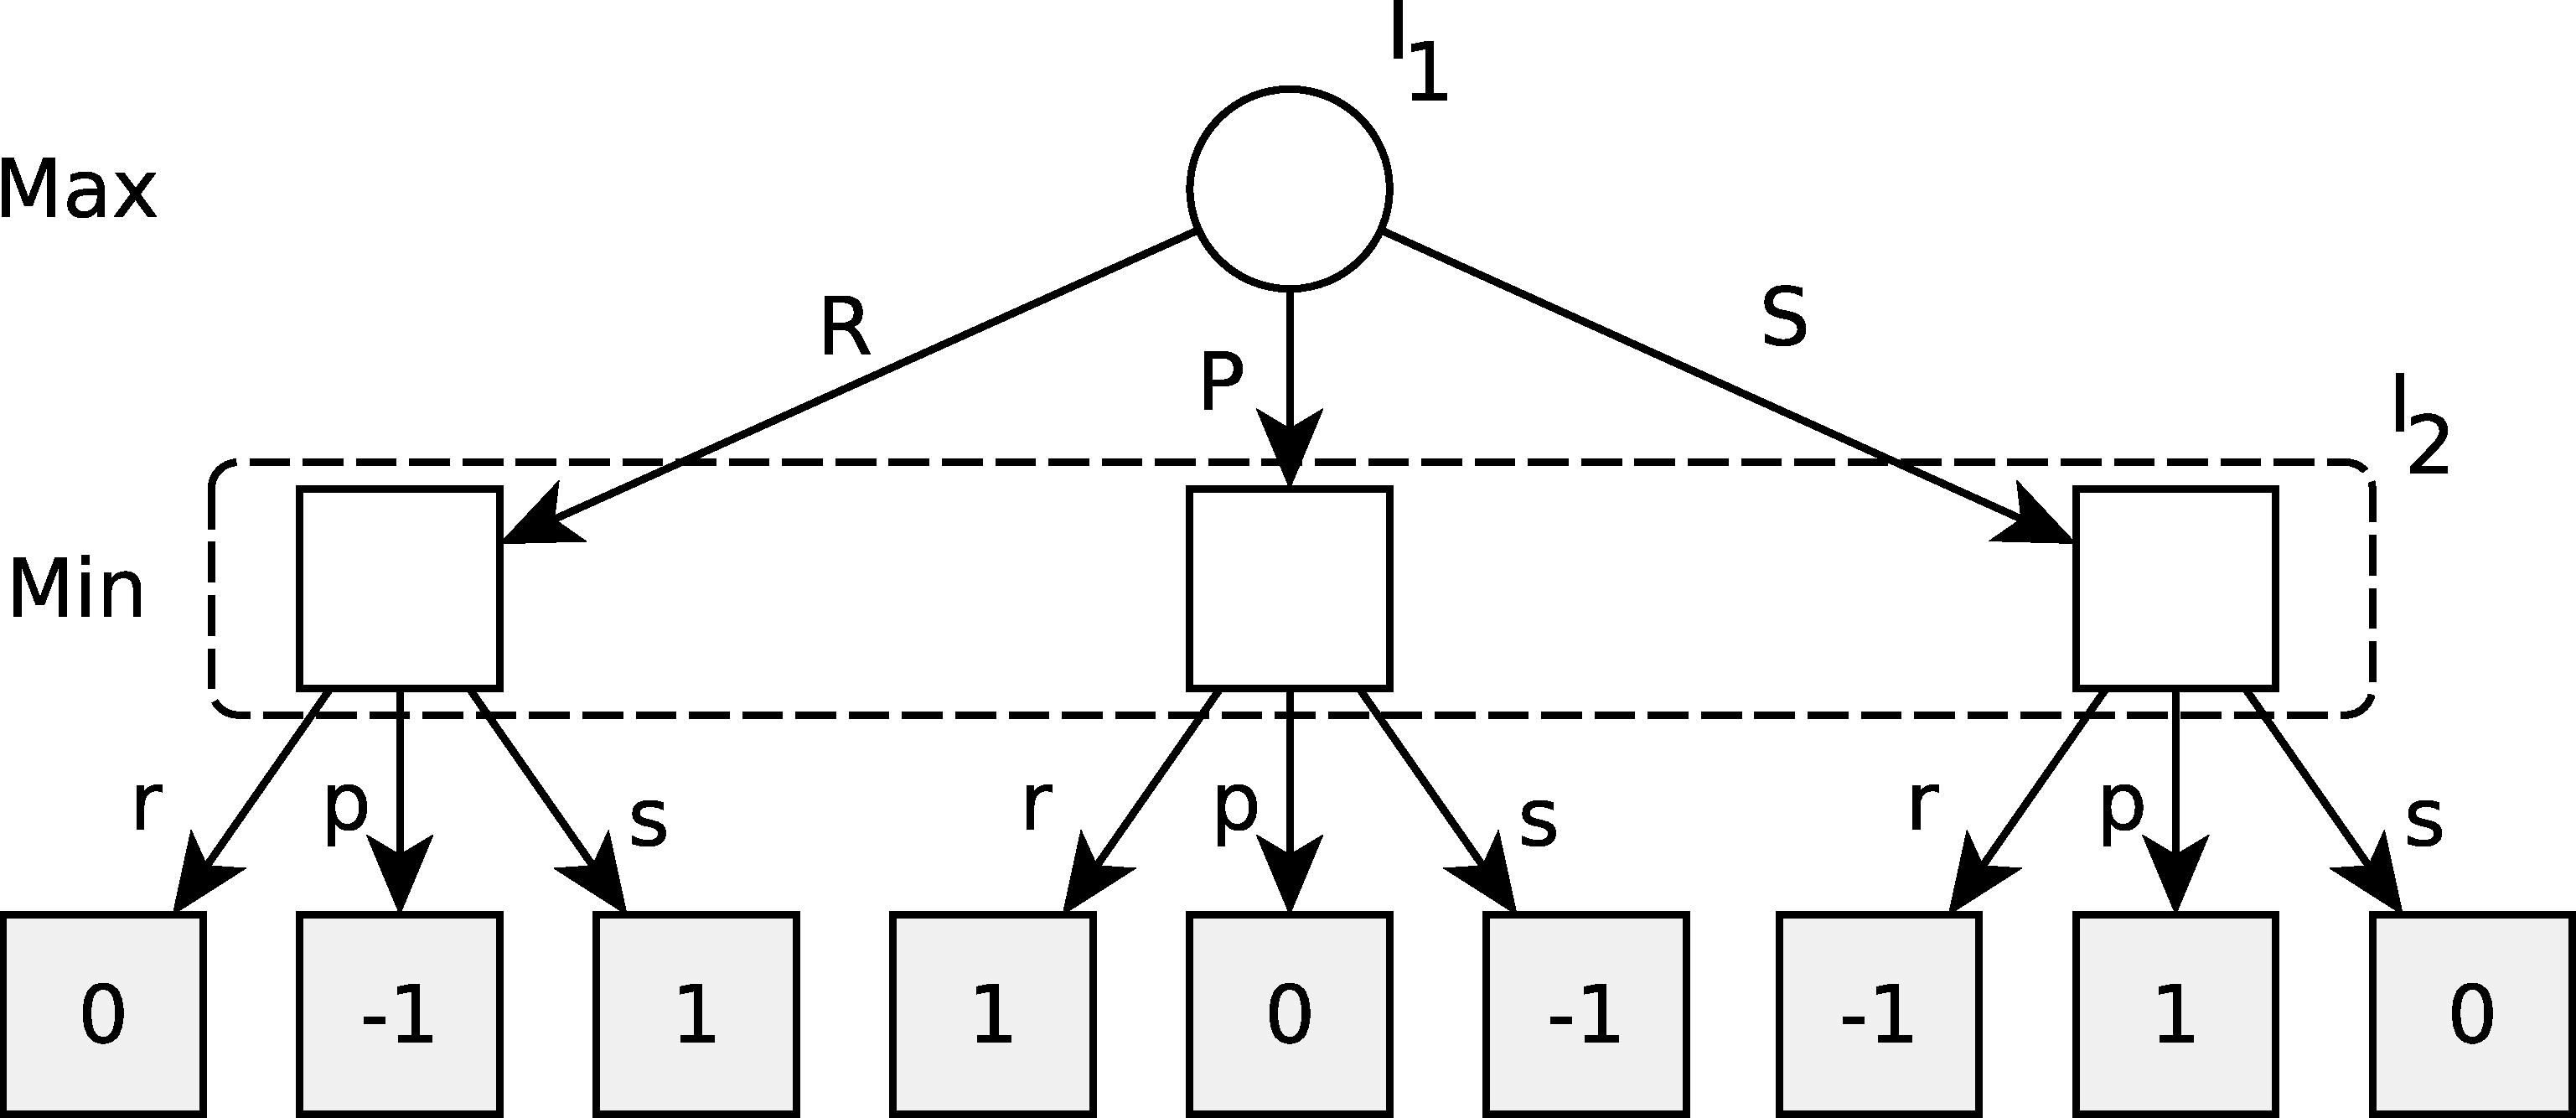
\includegraphics[width=0.6\textwidth]{figures/rps-new} \\
\end{tabular}
\end{center}
\caption{The matrix game of Rock, Paper, Scissors (left) and its equivalent extensive-form game representation (right). The extensive
game has four states, two information sets ($I_1$ and $I_2$),
and nine terminal histories: $\{ Rr, Rp, Rs, Pr, Pp, Ps, Sr, Sp, Ss \}$. \label{fig:rps-equiv}}
\end{figure}


